
\documentclass{article}

\usepackage{graphicx}
\usepackage{float}
\usepackage{geometry}
\usepackage{caption}
\usepackage{booktabs}
\usepackage{hyperref}

\geometry{margin=1in}
\graphicspath{{plots/}{plots_v2/}}

\title{Automated Materials Screening Report}
\author{AG2 Multi-Agent System}
\date{\today}

\begin{document}
\maketitle

\begin{abstract}
This paper investigates inorganic materials suitable as high-voltage protective barrier coatings near power lines. Our selection criteria focused on materials with energy above hull between 0.0 and 0.05 eV/atom, band gap between 3.0 and 20.0 eV, and density between 3.0 and 10.0 g/cm$^3$, excluding toxic elements such as Pb, Cd, and Hg. 
\end{abstract}
\section{Introduction}
High-voltage power lines require robust protective coatings to ensure operational safety and longevity. Inorganic materials with high band gaps and stability parameters, such as low energy above hull values, hold potential for such applications due to their insulative properties and environmental resistance.

\section{Methods}
We explored the Materials Project database to identify materials that match predefined criteria of stability and non-toxicity. We utilized parameters including energy above hull (0.0 to 0.05 eV/atom), wide band gaps (3.0 to 20.0 eV), and densities (3.0 to 10.0 g/cm$^3$), while excluding compounds containing toxic elements Pb, Cd, and Hg. Data visualization was conducted using scatter plots and histograms to assess property distributions and correlations.

\section{Results}
We retrieved 100 materials meeting the specified constraints. The analysis revealed strong clustering in the stable and near-stable ranges for energy above hull, predominantly wide band gaps, and density distributions that align with the criteria:

\begin{figure}[H]
\centering
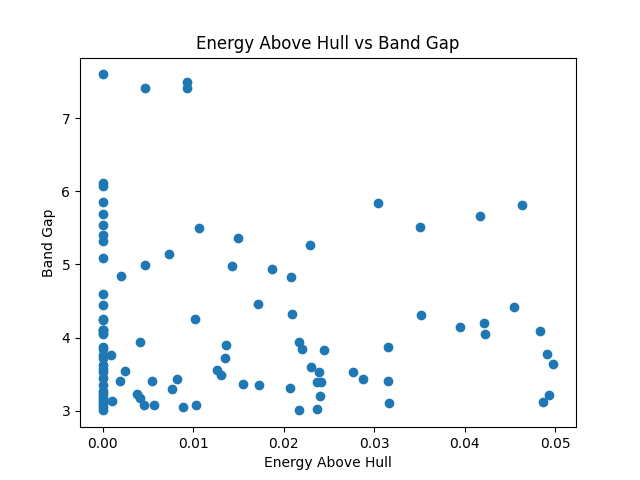
\includegraphics[width=0.8\textwidth]{plot_1_energy_above_hull_vs_band_gap.png}
\caption{Scatter plot of energy above hull vs band gap.}
\end{figure}

\begin{figure}[H]
\centering

\includegraphics[width=0.8\textwidth]{plot_2_density_vs_band_gap.png}
\caption{Scatter plot showing density vs band gap.}
\end{figure}

\begin{figure}[H]
\centering

\includegraphics[width=0.8\textwidth]{plot_3_density_vs_energy_above_hull.png}
\caption{Scatter plot of density vs energy above hull.}
\end{figure}

\begin{figure}[H]
\centering

\includegraphics[width=0.8\textwidth]{plot_4_histogram_of_energy_above_hull.png}
\caption{Histogram of energy above hull distribution.}
\end{figure}

\begin{figure}[H]
\centering

\includegraphics[width=0.8\textwidth]{plot_5_histogram_of_band_gap.png}
\caption{Histogram of band gap distribution.}
\end{figure}

\section{Discussion}
The retrieved inorganic materials exhibit properties well-suited for high-voltage applications, demonstrating sufficient stability and insulative performance. The predominance of materials with near-zero energy above hull suggests high thermodynamic stability. The distribution patterns observed in the histograms confirm that the selected ranges for band gaps and densities are appropriate for identifying materials with desired electrical insulation properties.

\section{Conclusion}
The study successfully identified 100 inorganic materials within the designated criteria suitable for potential use as high-voltage protective barrier coatings. These findings support the continued exploration of inorganic compounds with similar properties to enhance the development of durable and efficient barrier materials in electrical infrastructure.


\end{document}
